\documentclass[a4paper, 12pt]{article}

\usepackage{charter}
\usepackage{makeidx}
\usepackage{fancyhdr}
\usepackage{hyperref}
\usepackage[utf8]{inputenc}
\usepackage{graphicx}
\usepackage[left=2cm, right=2cm]{geometry}
\usepackage{latexsym}
\usepackage{amsmath, amsthm, amssymb}
\usepackage{rotating}


\begin{titlepage}
\title{Domain Model}
\author{Release 0.6}
\date{\today \\Firenze \\\begin{figure}[h] \centering

\includegraphics[width=0.2\textwidth]{../../../images/logokiwi.png} 
\end{figure}
}
\end{titlepage}

\pagestyle{fancy}

\begin{document}

\maketitle

\newpage

\section*{Approvazione, redazione, lista distribuzione}
\begin{table}[h!]
  \begin{center}
    \begin{tabular}{| l | l | p{60mm} |}
    \hline
    \textbf{approvato da} & \textbf{il giorno} & \textbf{firma} \\
	\hline    
	Marco Tinacci &  &  \\
    \hline
    \end{tabular}
  \end{center}
\end{table}

\begin{table}[h!]
  \begin{center}
    \begin{tabular}{| l | l | p{60mm} |}
    \hline
    \textbf{redatto da} & \textbf{il giorno} & \textbf{firma} \\
    \hline
    Francesco Calabri &  &  \\
    \hline
	Manuele Paulantonio &  &  \\
    \hline    
	Massimo Nocentini &  &  \\
    \hline
    \end{tabular}
  \end{center}
\end{table}

\begin{table}[h!]
  \begin{center}
    \begin{tabular}{| l | l | p{60mm} |}
    \hline
    \textbf{distribuito a} & \textbf{il giorno} & \textbf{firma} \\
	\hline    
	Daniele Poggi &  &  \\
    \hline
	Niccol\'o Rogai &  &  \\
    \hline
	Marco Tinacci &  &  \\
    \hline
    \end{tabular}
  \end{center}
\end{table}

\newpage

\tableofcontents

\newpage

\section*{Introduzione}

\newpage

\section{Overall diagram}
\begin{figure}[h!] 
	\centering
	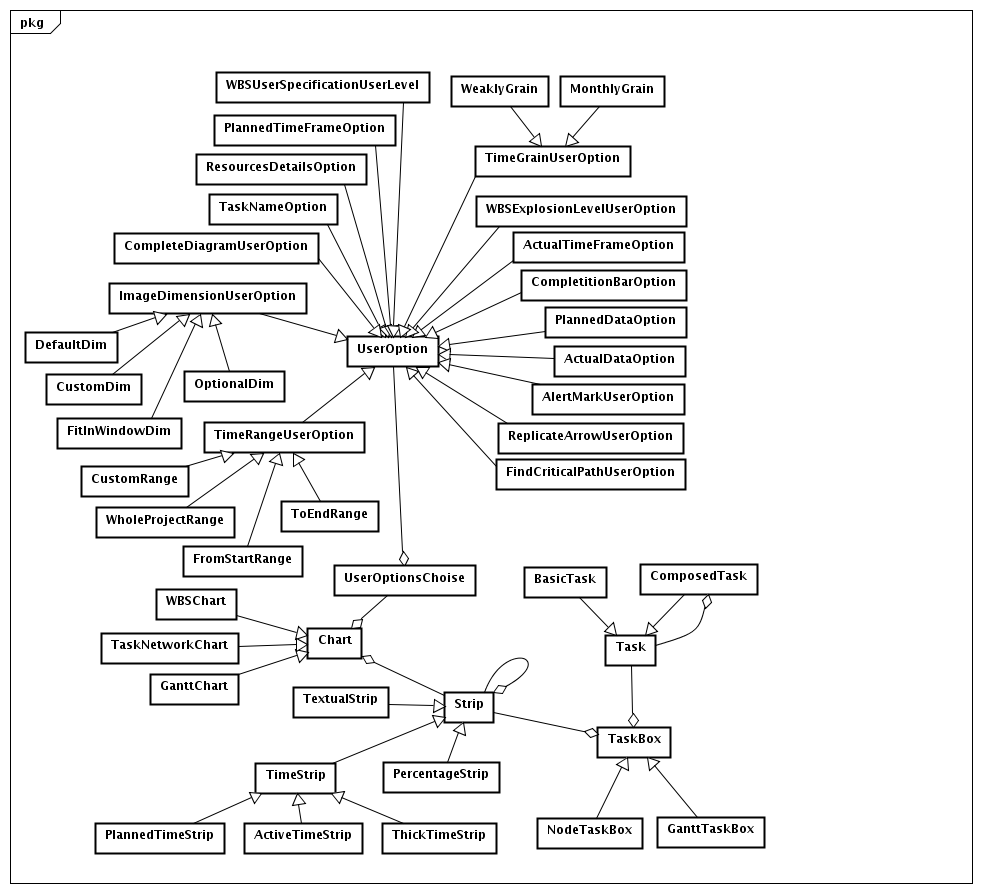
\includegraphics[width=1\textwidth]{../DomainModel.png}
	\caption{Overall UML diagram}
	\label{fig:overallDiagram} 
\end{figure}

Questo diagramma comprende tutti i concetti che abbiamo identificato durante la
prima iterazione del blocco di analisi. 

Nella figura abbiamo una visione di insieme che pu\`o essere utile a fini di
codifica e progettazione del piano delle prove. Finch\`e si rimane invece nella
sfera della progettazione (analisi inclusa) potrebbe produrre dei dubbi in
quanto propone molti concetti; mentre si sta cercando di raffinare le varie relazioni
secondo noi \`e necessaria una vista pi\`u in dettaglio di composizioni
di pochi concetti che sono legati tra loro, lasciando tutti gli altri ad una
loro commento separato.

Procediamo nel seguito del documento nella descrizione di piccole composizioni
in modo da chiarire i motivi per cui sono stati creati concetti e relazioni fra
essi.

% from here every document which is included with the input command must have a
% dedicated section whitin his body
\section{Task}
\label{sec:task}

\begin{figure}[h!] 
	\centering
	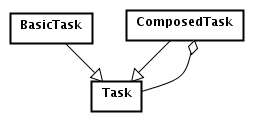
\includegraphics[width=0.4\textwidth]{../Milestone1-DomainModel/img/TaskDetail.png}
	\caption{task and its relations}
	\label{fig:task} 
\end{figure}

Molto probabilmente il concetto di \emph{Task} esiste gia nell'attuale
versione di \textbf{PMango 2.2.0}. Quello che abbiamo pensato \`e di introdurre
un \emph{glue layer} che ci permette di non apportare modifiche al codice
esistente di mango, ma lavorare con uno strato di intermezzo per essere il meno
intrusivi possibile e poter portare avanti il lavoro dipendendo solo dalle
nostri oggetti, facendo il minor riferimento al codice gia esistente.

Vogliamo rendere trasparente il concetto che un \emph{Task} sia un attivit\`a
singola (non scomponibile in sottoattivit\`a) che una attivit\`a scomposta. 

Costruiamo la relazione $\rightarrow$ che lega questi due concetti:
\begin{itemize}
  \item \emph{BasicTask} $\rightarrow$ attivit\`a di base, non ulteriormente
  scomponibili
  \item \emph{ComposedTask} $\rightarrow$ attivit\`a che sono composte da sotto
  attivit\`a
\end{itemize}
In questo modo possiamo trattare questi due tipi di attivit\`a in modo
interscambiabile e del tutto trasparente. Usando l'astrazione \emph{Task} non
ci importa se abbiamo una attivit\`a base o composta, in quanto cosi le abbiamo
portate ad avere interfaccie compatibili.

\section{TaskBox}
\label{sec:taskbox}

\begin{figure}[h!] 
	\centering
	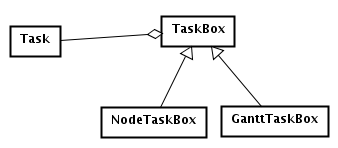
\includegraphics[width=0.5\textwidth]{../TaskBoxDetail.png}
	\caption{taskbox and its specializations}
	\label{fig:taskbox} 
\end{figure}

Il \emph{TaskBox} \`e la rappresentazione grafica di un
\emph{Task} (\autoref{fig:task}). Questo concetto astrae su queste
specializzazioni:
\begin{itemize}
\item \emph{GanttTaskBox} che ci permetter\`a di costruire la rappresentazione
in un \emph{GanttChart} conformi alle norme fissate nel documento di specifica.

\item \emph{NodeTaskBox} che ci permetter\`a di costruire la rappresentazione
in un \emph{WBSChart} e in \emph{TaskNetworkChart} alle norme fissate nel 
documento di specifica.
\end{itemize}

Abbiamo usato il principio di incapsulare il concetto che varia, modellando il
concetto astratto di \emph{TaskBox} per avere questi vantaggi:
\begin{itemize}
  \item non legare un \emph{Chart} specifico a una rappresentazione specifica
  \item aggiungere una nuova rappresentazione consiste nel modellarla e
  dichiarare che si tratta di una specializzazione di \emph{TaskBox}
  \item potremo cambiare a runtime il tipo di rappresentazione voluta nel
  disegno di un \emph{Chart}, magari inserire in un \emph{WBSChart} una
  rappresentazione pensata per i \emph{GanttChart}
\end{itemize}
\section{Strip}
\label{sec:strip}

\begin{figure}[h!] 
	\centering
	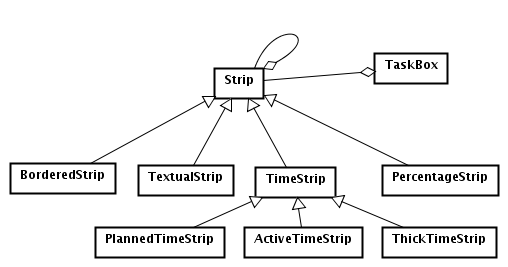
\includegraphics[width=0.7\textwidth]{../Milestone1-DomainModel/img/StripDetail.png}
	\caption{kinds of strips}
	\label{fig:strip} 
\end{figure}

La \emph{Strip} modella il concetto di ''striscia'': lo possiamo vedere come il
building block di pi\`u basso livello di tutta la nostra analisi. Si possono
osservare queste relazioni:
\begin{description}
  \item[TaskBox composition] \emph{TaskBox} contiene delle \emph{Strip},
  indipendentemente dalla rappresentazione dedicata ad uno specifico \emph{Chart}. Abbiamo costruito
  questa relazione in quanto per costruire un \emph{TaskBox} sar\`a sufficiente
  comporre un insieme di strip, tante quante sono necessarie per la corretta
  visualizzazione del \emph{Chart} che si sta disegnando.
  \item[russian doll] \emph{Strip} contiene a sua volta delle \emph{Strip}:
  questo \`e un concetto che pensiamo posso essere molto potente. Vogliamo rendere la
  \emph{Strip} un contenitore trasparente rispetto ad oggetti del suo stesso
  tipo. Questo ci permetter\`a di disegnare \emph{Strip} annidate, decidendo a
  runtime sia la \textbf{profondit\`a} di annidamento sia l'\textbf{ordine} con
  cui vengono annidate. Otteniamo cosi l'effetto di \emph{russian doll}, 
  dedicandoci a modellare solo alcune semplici specializzazioni di \emph{Strip},
  necessarie per l'implementazione delle notazioni richieste nel documento di specifica,
  limitandoci poi ad ottenere rappresentazioni complesse annidando quelle
  semplici.
  \item[specializations] abbiamo un primo livello di specializzazione:
  \begin{itemize}
    \item \emph{PercentageStrip} rappresenta un quantit\`a (l'intera
    \emph{Strip}) e la percentuale di comletamento (una parte di \emph{Strip}
    di colore diverso). Pu\`o essere composta da un \emph{GanttTaskBox} per
    indicare la percentuale di completamento relativa al \emph{Task}
    rappresentato.
    
    \item \emph{TextualStrip} permette di inserire delle stringhe di caratteri
    all'interno della \emph{Strip}. Questa possiamo utilizzarla ad esempio nel
    \emph{GanttChart} sulla destra della relativa \emph{TaskBox} per indicare
    l'effort oppure le risorse.
    
    \item \emph{BorderedStrip} permette di costruire un bordo, in modo che
    possiamo implementare la notazione per \emph{field} come richiesto per
    \emph{NodeTaskBox}
    
    \item \emph{TimeStrip} permettono di rappresentare informazioni relative a
    un intervallo di tempo. Queste sono i building blocks per
    \emph{GanttChart}. Possiamo specializzare ulteriormente questo concetto:
    \begin{itemize}
      \item \emph{PlannedTimeStrip} per costruire la parte superiore del
      \emph{GanttTaskBox} cdns
      \item \emph{ActualTimeStrip} per costruire la parte inferiore del
      \emph{GanttTaskBox} cdns      
      \item \emph{ThickTimeStrip} per costruire la parte superiore del
      \emph{GanttTaskBox} nel caso la rappresentazione sia di un
      \emph{ComposedTask} cdns
    \end{itemize}
  \end{itemize}
\end{description}

\section{Chart}
\label{sec:chart}

\begin{figure}[h!] 
	\centering
	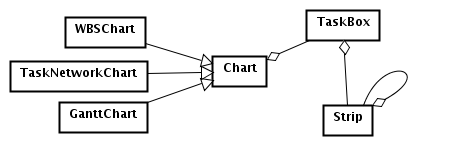
\includegraphics[width=0.6\textwidth]{../ChartDetail.png}
	\caption{chart and building blocks}
	\label{fig:chart} 
\end{figure}

Il \emph{Chart} modella il concetto di grafico generico. Per implementare la
specifica abbiamo queste specializzazioni:
\begin{itemize}
  \item \emph{GanttChart} che permette di avere la rappresentazione delle
  attivit\`a nel tempo
  \item \emph{WBSChart} per avere una vista gerarchica delle attivit\`a e di
  come sono state raffinate e decomposte in sotto attivit\`a
  \item \emph{TaskNetworkChart} per rappresentare le dipendenze di tipo
  \emph{finish-to start} fra coppie di attivit\`a
\end{itemize}

Per costruire un \emph{Chart} \`e sufficiente assemblare \emph{TaskBox} in base
ad alcune preferenze del client che richiede la generazione.

\end{document}